\begin{figure}[htb]
    \centering
    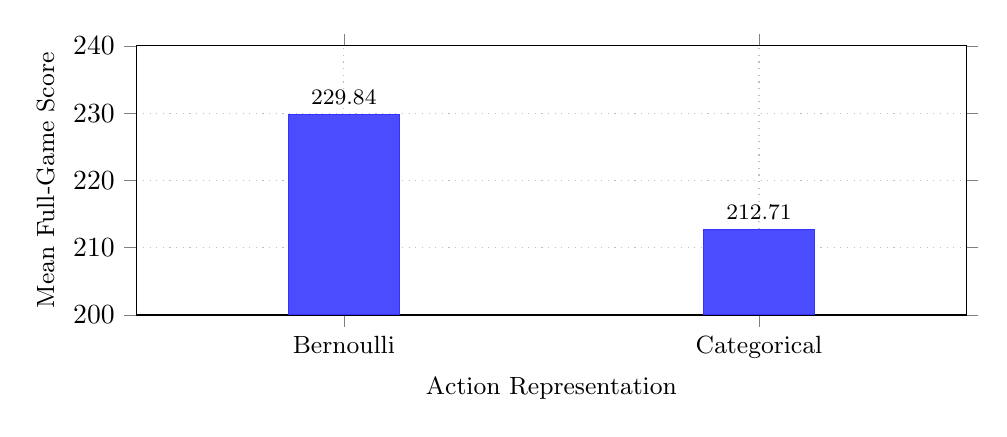
\begin{tikzpicture}
        \begin{axis}[
                ybar,
                width=\columnwidth,
                height=5cm,
                xlabel={Action Representation},
                ylabel={Mean Full-Game Score},
                symbolic x coords={Bernoulli, Categorical},
                xtick=data,
                xticklabel style={font=\small},
                ylabel style={font=\small},
                xlabel style={font=\small},
                bar width=40pt,
                ymin=200, ymax=240,
                grid=both,
                grid style={dotted},
                tick align=outside,
                nodes near coords,
                nodes near coords style={font=\footnotesize, anchor=south},
                enlarge x limits=0.5,
            ]

            \addplot[
                fill=blue!70!white,
                draw=blue!80,
                error bars/.cd,
                y dir=both,
                y explicit
            ] coordinates {
                    (Bernoulli, 229.84)
                    (Categorical, 212.71)
                };

        \end{axis}
    \end{tikzpicture}
    \caption{Performance comparison: Bernoulli vs Categorical action representation}
    \label{fig:bernoulli-vs-categorical}
\end{figure}

\begin{figure}[htb]
    \centering
    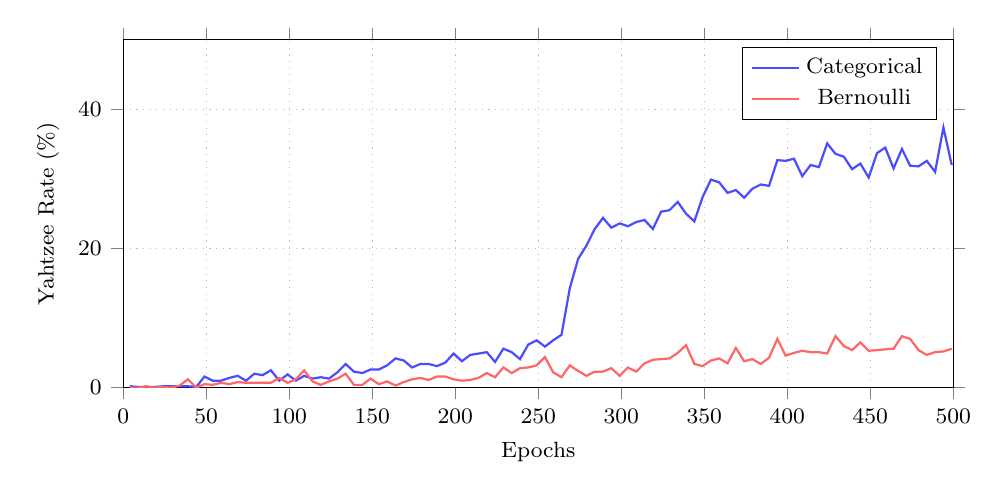
\begin{tikzpicture}
        \begin{axis}[
                width=\columnwidth,
                height=6cm,
                xlabel={Epochs},
                ylabel={Yahtzee Rate (\%)},
                xmin=0, xmax=500,
                ymin=0, ymax=50,
                grid=both,
                grid style={dotted},
                tick align=outside,
                tick label style={font=\footnotesize},
                label style={font=\footnotesize},
                legend style={at={(0.98,0.98)},anchor=north east,font=\footnotesize}
            ]

            % Categorical (glowing-sweep-1)
            \addplot[
                thick,
                blue!70!white
            ] coordinates {
                    (4, 0.2) (9, 0.1) (14, 0.1) (19, 0.1) (24, 0.2) (29, 0.2) (34, 0.2) (39, 0.2) (44, 0.1) (49, 1.6) (54, 1) (59, 1) (64, 1.4) (69, 1.7) (74, 1) (79, 2) (84, 1.8) (89, 2.5) (94, 1) (99, 1.9) (104, 1) (109, 1.7) (114, 1.3) (119, 1.5) (124, 1.3) (129, 2.2) (134, 3.4) (139, 2.3) (144, 2.1) (149, 2.6) (154, 2.6) (159, 3.2) (164, 4.2) (169, 3.9) (174, 2.9) (179, 3.4) (184, 3.4) (189, 3.1) (194, 3.6) (199, 4.9) (204, 3.8) (209, 4.7) (214, 4.9) (219, 5.1) (224, 3.7) (229, 5.6) (234, 5.1) (239, 4.1) (244, 6.2) (249, 6.8) (254, 5.9) (259, 6.8) (264, 7.6) (269, 14.3) (274, 18.5) (279, 20.4) (284, 22.8) (289, 24.4) (294, 23) (299, 23.6) (304, 23.2) (309, 23.8) (314, 24.1) (319, 22.8) (324, 25.3) (329, 25.5) (334, 26.7) (339, 25) (344, 23.9) (349, 27.4) (354, 29.9) (359, 29.5) (364, 28) (369, 28.4) (374, 27.3) (379, 28.6) (384, 29.2) (389, 29) (394, 32.7) (399, 32.6) (404, 32.9) (409, 30.4) (414, 32) (419, 31.7) (424, 35.1) (429, 33.6) (434, 33.2) (439, 31.4) (444, 32.2) (449, 30.2) (454, 33.7) (459, 34.5) (464, 31.5) (469, 34.3) (474, 31.9) (479, 31.8) (484, 32.6) (489, 31) (494, 37.4) (499, 32)
                };
            \addlegendentry{Categorical}

            % Bernoulli (helpful-sweep-2)
            \addplot[
                thick,
                red!60!white
            ] coordinates {
                    (4, 0) (9, 0) (14, 0.2) (19, 0) (24, 0.1) (29, 0) (34, 0.3) (39, 1.2) (44, 0) (49, 0.5) (54, 0.4) (59, 0.7) (64, 0.5) (69, 0.8) (74, 0.7) (79, 0.7) (84, 0.7) (89, 0.7) (94, 1.4) (99, 0.7) (104, 1.2) (109, 2.5) (114, 0.9) (119, 0.4) (124, 0.9) (129, 1.3) (134, 2) (139, 0.4) (144, 0.4) (149, 1.3) (154, 0.5) (159, 0.9) (164, 0.3) (169, 0.8) (174, 1.2) (179, 1.4) (184, 1.1) (189, 1.6) (194, 1.6) (199, 1.2) (204, 1) (209, 1.1) (214, 1.4) (219, 2.1) (224, 1.5) (229, 2.9) (234, 2.1) (239, 2.8) (244, 2.9) (249, 3.2) (254, 4.4) (259, 2.2) (264, 1.5) (269, 3.2) (274, 2.4) (279, 1.7) (284, 2.3) (289, 2.3) (294, 2.8) (299, 1.7) (304, 2.9) (309, 2.3) (314, 3.5) (319, 4) (324, 4.1) (329, 4.2) (334, 5) (339, 6.1) (344, 3.4) (349, 3.1) (354, 3.9) (359, 4.2) (364, 3.5) (369, 5.7) (374, 3.8) (379, 4.1) (384, 3.4) (389, 4.3) (394, 7) (399, 4.6) (404, 5) (409, 5.3) (414, 5.1) (419, 5.1) (424, 4.9) (429, 7.4) (434, 6) (439, 5.4) (444, 6.5) (449, 5.3) (454, 5.4) (459, 5.5) (464, 5.6) (469, 7.4) (474, 7) (479, 5.4) (484, 4.7) (489, 5.1) (494, 5.2) (499, 5.6)
                };
            \addlegendentry{Bernoulli}

        \end{axis}
    \end{tikzpicture}
    \caption{Learning Yahtzee with different action representations}
    \label{fig:action-yahtzee-learning}
\end{figure}